\documentclass[twocolumn, 12pt]{article}
\usepackage[utf8]{inputenc}
\usepackage{amsmath}
\usepackage{marvosym}
\usepackage{textcomp}
\usepackage{geometry}
\usepackage{array}
\usepackage{wrapfig}
\usepackage{multirow}
\usepackage{graphicx}
\usepackage{float}
\usepackage{wrapfig}
\usepackage{caption}
\usepackage{amssymb}
\usepackage{multicol}

\geometry{a4paper, margin=.75in}



\begin{document}
\small
\pagestyle{empty}

\section*{Electricity and Magnetism}
\subsection*{Equations}


\begin{equation*}
    \boxed{\textbf{F}_e = k_e \frac{|q_1q_2|}{r^2}\hat{r}}  \hspace{15pt}  k_e \triangleq \frac{1}{4\pi\epsilon_0} = 9(10^9) \frac{Nm^2}{C^2}
\end{equation*}

\begin{equation*}
    \textbf{F}_e = q\textbf{E}   \hspace{15pt}   \textbf{E}_{\texttt{net}} = \sum_i k_e\frac{q_i}{r_i^2}  \hat{r}  = \int k_e \frac{dq}{r^2} \hat{r}
\end{equation*}

\begin{equation*}
     \lambda = \frac{dq}{dL} \hspace{15pt} \eta = \frac{dq}{dA} \hspace{15pt} \rho =\frac{dq}{dV} \hspace{15pt} \textbf{E}_{\texttt{plane}} = \frac{|\eta|}{2\epsilon_0}
\end{equation*}

\begin{equation*}
    \textbf{E}_c = \frac{Q}{\epsilon_0 A}   \hspace{15pt}  \Phi_s \equiv \oint \textbf{E} \bullet d\textbf{A} = \frac{q_{\texttt{in}}}{\epsilon _0}
\end{equation*}

\begin{equation*}
    U_e = \sum^{\texttt{all}}_{\texttt{pairs}} k_e \frac{q_iq_j}{r_{ij}}   \hspace{15pt}  V \triangleq \frac{U_{q + \texttt{sources}}}{q}
\end{equation*}

\begin{equation*}
    \Delta V = -\int_a^b \textbf{E} \bullet d\textbf{s}   \hspace{15pt}   U=qV \hspace{15pt}  \textbf{E} = -\vec{\nabla} V
\end{equation*}

\begin{equation*}
    W = q\texttt{E}_s\Delta s \hspace{15pt}  \Delta U =-q\texttt{E}_s\Delta s \hspace{15pt} \Delta V = - \texttt{E}_s \Delta s
\end{equation*}

\begin{equation*}
    C \triangleq \frac{Q}{\Delta V } \hspace{15pt} C_c = \frac{\epsilon_0 A}{d}  \hspace{15pt}  U_c= \frac{1}{2} C \Delta V^2
\end{equation*}

\begin{equation*}
    I(t) = - \frac{dQ}{dt} \hspace{15pt} J \triangleq \frac{I}{A}  \hspace{15pt} J_{\text{total}} = J_{\text{portion}}
\end{equation*}

\begin{equation*}
    \boxed{ J=\sigma \texttt{E} \hspace{8pt} \Longleftrightarrow \hspace{8pt}  V=IR}
\end{equation*}

\begin{equation*}
    R = \frac{L}{\sigma A} = \frac{\rho L}{A} \hspace{15pt} \rho \sigma =1
\end{equation*}

\begin{equation*}
    P \triangleq \frac{dE}{dt} = IV = I^2R = \frac{V^2}{R}
\end{equation*}

\begin{equation*}
    \text{Kirchoff: }\boxed{  \Sigma I_{\texttt{in}} = \Sigma I_{\texttt{out}}  \hspace{10pt}  \Sigma V_{\texttt{closed loop}} =0}
\end{equation*}

\begin{equation*}
    \text{Biot-Savart Law:  } \boxed{\textbf{B} = \frac{\mu_0 I}{4\pi} \int \frac{d\vec{s} \times \hat{r}}{r^2} }
\end{equation*}

\begin{equation*}
    \vec{\mu} \triangleq N I \vec{A} \hspace{15pt} \vec{A} = \hat{n}A \hspace{15pt} \tau = \vec{\mu} \times \textbf{B} \hspace{15pt} \tau_L =\frac{L}{R}  
\end{equation*}

\begin{equation*}
    \textbf{B}_{\text{solenoid}}(t) = \mu_0 nI(t) \hspace{15pt} n=\frac{N}{l} \hspace{15pt} \textbf{F}_B = q\textbf{v}_+ \times \textbf{B}
\end{equation*}

\begin{equation*}
    \textbf{F}_B =I\textbf{L}\times \textbf{B} \hspace{15pt} \Phi_B = \int \textbf{B} \bullet d\vec{A} 
\end{equation*}

\begin{equation*}
   \boxed{ \varepsilon_{ind} = \oint\textbf{E} \bullet d\vec{s} = -\frac{d\Phi_B}{dt} =-\frac{d}{dt} \int \textbf{B} \bullet d\vec{A}}
\end{equation*}

\begin{equation*}
    \varepsilon_L = -L\frac{dI}{dt} \hspace{15pt} \Phi_B =LI \hspace{15pt} P_L = I\varepsilon_L 
\end{equation*}

\begin{equation*}
    \omega =2\pi f \hspace{15pt} \omega = \sqrt{\frac{1}{LC}} \hspace{15pt} I_{max}= Q_0 \omega
\end{equation*}

\begin{equation*}
    Q(t) = Q_0cos(\omega t) \hspace{15pt} I(t) = I_{max}sin(\omega t)
\end{equation*}






\subsection*{Charging Capacitor}
\begin{equation*}
    q(t) = q_\infty (1-e^{-t/\tau}) \hspace{15pt}  I(t) = \frac{dq}{dt} = I_0e^{-t/\tau}
\end{equation*}




\subsection*{Discharging Capacitor}
\begin{equation*}
    q(t) = q_0 (e^-t/\tau ) \hspace{15pt}  I(t) = \frac{dq}{dt} -I_0 e^{-t/\tau }
\end{equation*}








\subsection*{Series Circuits}
\begin{equation*}
    R_T = R_1 + R_2+ \dotsc +R_n
\end{equation*}

\begin{equation*}
    \frac{1}{C_T} = \frac{1}{C_1} + \frac{1}{C_2}+\dotsc+\frac{1}{C_n}
\end{equation*}

\begin{equation*}
    Q_1 = Q_2 = \dotsc = Q_n
\end{equation*}

\begin{equation*}
    L_T = L_1 + L_2 + \dotsc L_n
\end{equation*}





\subsection*{Parallel Circuits}
\begin{equation*}
    \frac{1}{R_T} = \frac{1}{R_1} + \frac{1}{R_2} + \dotsc + \frac{1}{R_n}
\end{equation*}

\begin{equation*}
    C_T = C_1 + C_2 + \dotsc +C_n
\end{equation*}

\begin{equation*}
    Q_T = Q_1 + Q_2 +\dotsc + Q_n
\end{equation*}

\begin{equation*}
    \frac{1}{L_T} = \frac{1}{L_1} + \frac{1}{L_2} + \dotsc + \frac{1}{L_n}
\end{equation*}






\subsection*{Using Gauss' Law}
\begin{enumerate}
    \item Find the direction of the electric field
    \item Choose a Gaussian Surface that satisfies the following criteria for all points on the surface:
    \begin{itemize}
        \item The electric field has a constant value
        \item The electric field is perpendicular to the surface
    \end{itemize}
    This allows the integral to simplify to:
    \begin{equation*}
       \boxed{ \Phi_E =\oint \textbf{E} \bullet d\vec{A} \hspace{8pt} \Longrightarrow \hspace{8pt} \textbf{E} = \frac{q_{\texttt{in}}}{\epsilon_0 A_{ \texttt{G.S.}}}}
    \end{equation*}
    \item Find the total charge inside the Gaussian Surface (\(q_{\texttt{in}}\))
\end{enumerate}



\subsection*{Using Ampère's Law}
\begin{enumerate}
    \item Using symmetry, sketch \textbf{B}
    \item Draw an Amperian loop passing through point of interest (choose such that it results \(\textbf{B} \bullet d\vec{s}\) or 0)
    \item Find net current through the loop
    \item Apply Ampère's Law \\
    \begin{equation*}
        \boxed{ \oint \textbf{B} \bullet d\vec{s} = \mu_0I_{net}}
    \end{equation*}
\end{enumerate}




\subsection*{Motional \(\varepsilon\)MF}
\begin{figure}[h]
    \centering
    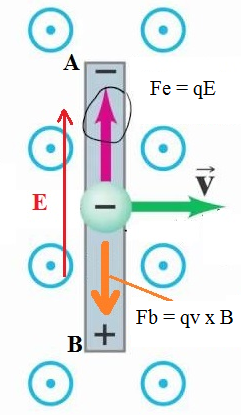
\includegraphics[scale=0.5, angle=90]{Motional EMF.png}
\end{figure}



\begin{enumerate}
    \item Motion of bar causes \(\textbf{F}_B\). \(\textbf{F}_B=q\textbf{v} \times \textbf{B}\)
    \item \(\textbf{F}_B\) pushes positives to one end. The negatives go to the other end.
    \item This causes a voltage between the two ends. \(\Delta V = -\int \textbf{E} \bullet d\vec{l} = El\)
    \item \(\textbf{F}_B =\textbf{F}_E  \hspace{5pt} \Longrightarrow  \hspace{5pt} qvB=qE \hspace{5pt} \Longrightarrow \hspace{5pt} vB=E \)
    \item \( \Delta V = \varepsilon = vBL\)
\end{enumerate}
\begin{center}
    The potential difference across the conductor \(\equiv\) motional emf
\end{center} 

\begin{equation*}
    P_{in} = \textbf{F}v_0 = \left(\frac{v_0\textbf{B} L}{R} \right)  v_0\textbf{B} L = I^2R = P_{out}
\end{equation*}





\subsection*{Lenz's Law}
\begin{equation*}
    \varepsilon_{ind} = \hspace{10pt} \frac{d\textbf{B}}{dt}A \hspace{10pt} \text{OR} \hspace{10pt} B \frac{dA}{dt}
\end{equation*}

\begin{enumerate}
    \item Left thumb towards increasing \textbf{B}
    \item Right thumb anti-parallel to left thumb 
    \item Right hand finger curl is direction of \(I_{ind}\)
\end{enumerate}




\subsection*{Maxwell's Laws}
\begin{enumerate}
    \item Gauss' Law
        \begin{equation*}
            \Phi_E = \oint \textbf{E} \bullet d\vec{A} = \frac{q_{in}}{\epsilon_0}
        \end{equation*}
    \item Gauss's Law for Magnetism
        \begin{equation*}
            \oint \textbf{B} \bullet d\vec{A} = 0
        \end{equation*}
    \item Faraday's Law
        \begin{equation*}
            \oint \textbf{E} \bullet d\vec{s} = -\frac{d \Phi_B}{dt}
        \end{equation*}
    \item Ampère-Maxwell Law 
        \begin{equation*}
            \oint \textbf{B} \bullet d\vec{s} = \mu_0 \left(I + \epsilon_0 \frac{d\Phi_E}{dt}  \right)
        \end{equation*}
\end{enumerate}
Plus bonus: 
\begin{itemize}
    \item Lorentz Force
        \begin{equation*}
            \textbf{F} = q_+(\textbf{E} +\textbf{v} \times \textbf{B})
        \end{equation*}
\end{itemize}





\subsection*{Waves}
\begin{equation*}
    \textbf{E}_{xx}= \epsilon_0 \mu_0 \textbf{E}_{tt} \hspace{15pt} \textbf{E}(x,t) = \textbf{E}_0 cos (kx-\omega t)
\end{equation*}


\begin{equation*}
    \textbf{B}_{xx} = \epsilon_0 \mu _0 \textbf{B}_{tt} \hspace{15pt} \textbf{B}(x,t) = \textbf{B}_0 cos (kx- \omega t)
\end{equation*}

\begin{equation*}
    \textbf{E}_{\text{max}}= \textbf{B}_{\text{max}}c \hspace{15pt} \omega =2\pi f \hspace{15pt} k \triangleq \frac{2\pi}{\lambda}
\end{equation*}

\begin{equation*}
    v = \lambda f \hspace{15pt} v = \frac{1}{\sqrt{\epsilon _0 \mu _0}} \triangleq c \hspace{15pt} 1= fT \hspace{15pt} f=\frac{E}{h}
\end{equation*}

\begin{equation*}
    U_E = \frac{1}{2} \epsilon_0 \textbf{E}_0^2  \hspace{15pt} U_B = \frac{1}{2\mu_0} \textbf{B}_0^2 \hspace{15pt} U_T = \epsilon_0 \textbf{E}^2
\end{equation*}

\begin{equation*}
    \textbf{S} \triangleq \frac{1}{\mu _0} \textbf{E} \times \textbf{B} \hspace{15pt} |\textbf{S}| = \frac{1}{A}\frac{dU}{dt} \hspace{15pt} \textbf{S}_{\text{max}} = \frac{\textbf{E}_0^2}{c\mu_0}
\end{equation*}

\begin{equation*}
    \textbf{S}_{\text{avg}}= \textit{I} = \frac{P}{A}= \frac{\textbf{E}_0^2}{2c\mu_0}= \frac{c\epsilon_0 \textbf{E}_0^2}{2}
\end{equation*}

\begin{equation*}
    \textit{I} = U_{\text{avg}} c \hspace{15pt} \textit{I}_{\text{point source}}= \frac{P_{\text{source}}}{4\pi r^2}
\end{equation*}


\subsection*{Radiation Pressure}
\begin{equation*}
    E = mc^2 \Longrightarrow m=\frac{E}{c^2}
\end{equation*}

\begin{equation*}
    p=mv \Longrightarrow p = \frac{E}{c^2}c= \frac{E}{c}
\end{equation*}

\begin{equation*}
    \textbf{F}=\frac{dp}{dt} = \frac{1}{c}\frac{dE}{dt} = \frac{1}{c}\textit{I}A
\end{equation*}

\begin{equation*}
    \textbf{F} = \frac{1}{c}\textit{I}A \hspace{15pt} \sigma = \frac{\textit{I}}{c}
\end{equation*}

\subsection*{Additional Notes}
\begin{itemize}
    \item Electric field lines point in the direction of decreasing electrical potential
    \item After a long time: 
    \begin{itemize}
        \item Capacitors behave like batteries
        \item Inductors/coils behave like wires
        \item Resistors 
    \end{itemize}
    \item Antiparallel currents repel, parallel currents attract
\end{itemize}








\end{document}